\documentclass{beamer}
\usefonttheme[onlymath]{serif}

\usepackage{amsfonts}

% Code Block Setting
\usepackage{listings}
\lstset{language=C,
numberstyle=\footnotesize,
basicstyle=\ttfamily\footnotesize,
numbers=left,
stepnumber=1,
frame=shadowbox,
breaklines=true}

\usetheme{Warsaw}
% \usecolortheme{dove}

% Add frame number and total frame number in footline
\defbeamertemplate*{footline}{shadow theme}{%
    \leavevmode%
    \hbox{\begin{beamercolorbox}[wd=.5\paperwidth,ht=2.5ex,dp=1.125ex,leftskip=.3cm plus1fil,rightskip=.3cm]{author in head/foot}%
            \usebeamerfont{author in head/foot}\hfill\insertshortauthor
        \end{beamercolorbox}%
        \begin{beamercolorbox}[wd=.4\paperwidth,ht=2.5ex,dp=1.125ex,leftskip=.3cm,rightskip=.3cm plus1fil]{title in head/foot}%
            \usebeamerfont{title in head/foot}\insertshorttitle\hfill%
        \end{beamercolorbox}%
        \begin{beamercolorbox}[wd=.1\paperwidth,ht=2.5ex,dp=1.125ex,leftskip=.3cm,rightskip=.3cm plus1fil]{title in head/foot}%
            \hfill\insertframenumber\,/\,\inserttotalframenumber
    \end{beamercolorbox}}%
    \vskip0pt%
}

% Tikz related
\usepackage{tikz}
\usetikzlibrary{fit}
\usetikzlibrary{calc}
\usetikzlibrary{positioning}

% Number the figures
\setbeamertemplate{caption}[numbered]

% Add outline page at begining of each section
\AtBeginSection[]
{
    \begin{frame}<beamer>
        \frametitle{Outline}
        \tableofcontents[currentsection, hideallsubsections]
    \end{frame}
}

%%%%%%%%%%%%%%%%%%%%%%%%%%%%%%%%%%%%%%%%%%%%%

\title{MLbase: A Distributed Machine-learning System}
\author{
    Tim Kraska\inst{1},\\
	Rean Griffith\inst{2},\\
    Ameet Talwalkar\inst{3},\\
    John Duchi\inst{3},\\
    Michael J. Franklin\inst{3},\\
	Michael Jordan\inst{3}
}
\institute{
    \inst{1} Brown University
	\inst{2} VMware
	\inst{3} AMPLab, UC Berkeley
}
\date{
    \tiny{CIDR 2013. 6th Biennial Conference on Innovative Data Systems Research}\\
    \tiny{Presented by Ching-Yuan, Tsai}
}

\begin{document}
\begin{frame}
    \titlepage
\end{frame}

\section{Introduction}

\subsection{SIMD}
\begin{frame}
    \frametitle{SIMD}
	\begin{itemize}
		\item Single instruction multiple data
		\item without threads support
	\end{itemize}
\end{frame}


\subsection{VPU}
\begin{frame}
    \frametitle{VPU}
	\begin{itemize}
		\item Vector processing units 
		\item combine itstructions as vector	
	    \begin{figure}
			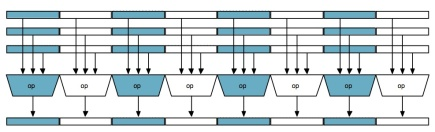
\includegraphics[scale=0.5]{figure/vpu.jpg}
		\end{figure}
	\end{itemize}
\end{frame}


\section{Architecture}

\subsection{Architecture}
\begin{frame}
    \frametitle{Architecture}
	\begin{figure}
		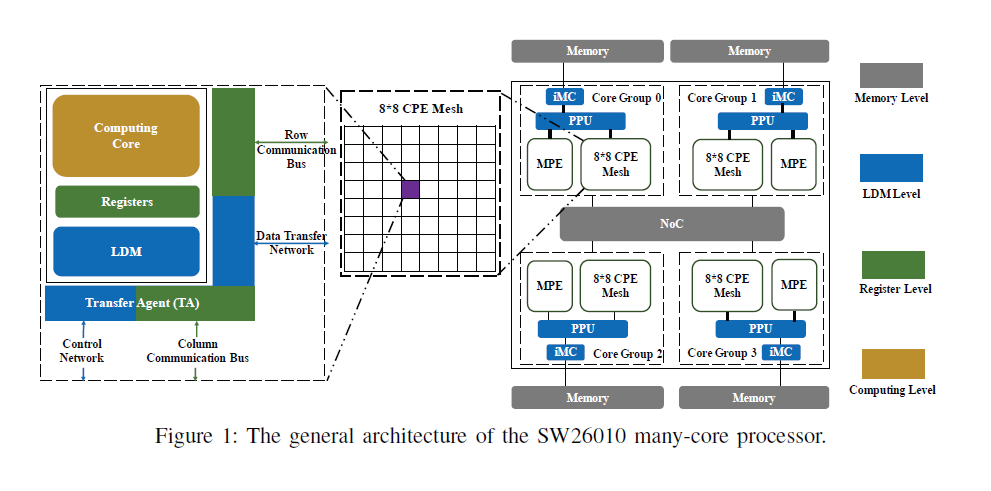
\includegraphics[scale=0.4]{figure/archi.PNG}
	\end{figure} 
\end{frame}

\subsection{Unique features}
\begin{frame}
    \frametitle{Unique features}
	\begin{itemize}
		\item Each CG has an MPE.
		\item Users can explicitly set the sizeof each CG's private memory space, and the size of shared memory space.  
		\item Support a 64kb user-controlled fast buffer for each computing cores. 
		\item Rigister communication between computing cores.
		\item Each computing core consists of two execution pipelines.  
	\end{itemize} 
\end{frame}

\subsection{Challenges}
\begin{frame}
    \frametitle{Challenges}
	\begin{itemize}
		\item Low memory bandwidth. 
		\begin{itemize}
			\item SW26010:36 GB/s for each CG, 144 GB/S for entire processor.  
			\item NVIDIA K80GPU: 480 GB/S for entire processor. 
		\end{itemize}
		\item CPEs do not have a shared buffer to rely on a fine-grained data sharing scheme. 
	\end{itemize}
\end{frame}

	


\section{Optimization}

\subsection{Hybrid CORDAC}
\begin{frame}
    \frametitle{Hybrid CORDAC}
		Cache-efficient algorithm recursive subdivision continues until 
		the problem size becomes small enough.
	\begin{itemize}
		\item Benefits of both iterative and recursive algorithms
		\item Asymptotic improvement in parallelism
		\item Highly optimizable base cases
	\end{itemize}
\end{frame}

\subsection{Optimizing Kernel Functions}
\begin{frame}
    \frametitle{Optimizing Kernel Functions}
	\begin{description}
		\item[Copy-optimization] Copy the data into local $b \times b$ 
			static arrays inside the kernel.
		\item[Loop Reordering] In flexible kernels, it is possible to change
			the looping order without hampering the correctness of the algorithm.
	\end{description}
\end{frame}

\subsection{Data Layout}
\begin{frame}
    \frametitle{Data Layout}
	\begin{figure}
		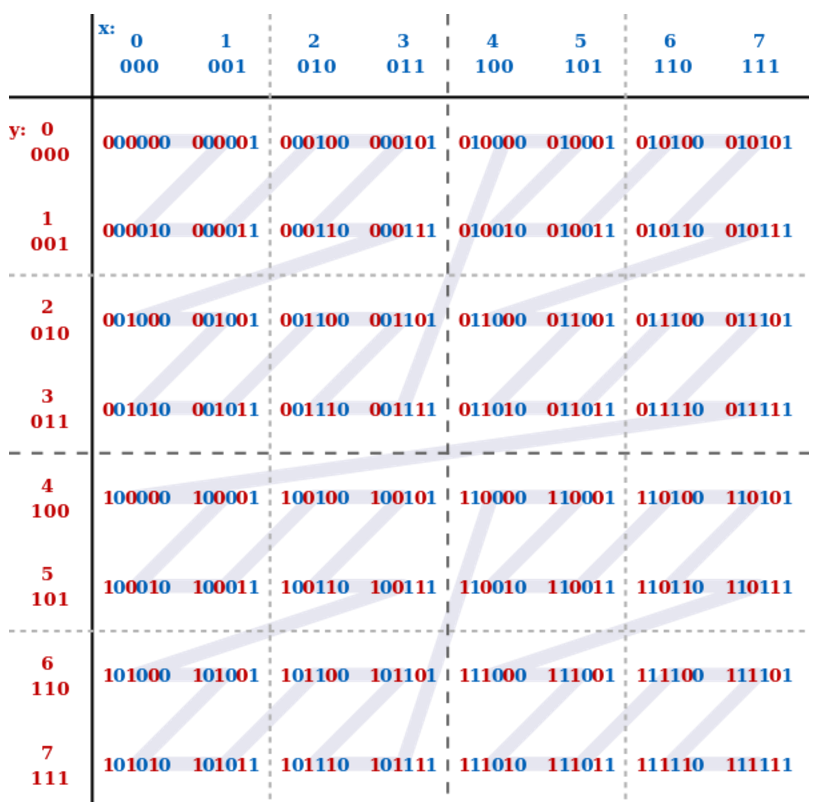
\includegraphics[scale=0.2]{figure/fig-z-morton.png}
	\end{figure}
	\begin{itemize}
		\item \textit{Z-Morton Row-Major}(ZM\_RM) layout is beneficial because
			it improves both temporal and spatial localities.
	\end{itemize}
\end{frame}

\subsection{Auto vs. Explicit Vectorization}
\begin{frame}
    \frametitle{Auto vs. Explicit Vectorization}
    It often vectorize the base-case of the dominating kernel.
	\begin{itemize}
		\item For example, $C_{\textit{loop}}$ is enough to get the 
			major share of the speedup.
	\end{itemize}
\end{frame}
\section{Conclusions}

\subsection{Conclusions}
\begin{frame}
	\frametitle{Conclusions}
	\begin{itemize}
		\item This paper proposed new format: block compressed common coordinate
			(BCCOO) to improve locality for accesses to the multiplied vector.
		\item Combine Matrix-based segmented sum/scan and BCCOO/BCCOO+ format to
			reduce the memory bandwidth.
		\item It improves at least 40\% preformance.
	\end{itemize}
\end{frame}
\end{document}
